\section{Case study - Design of Digital Keyword Spotter}
\label{sec:system_design}


%%% FIGURE: KWS ARCHITECTURE
%%% ------------------------
\begin{figure}[htbp]	
    %\centerline{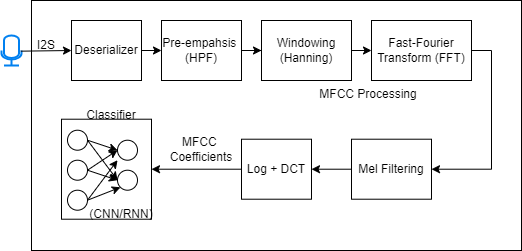
\includegraphics{figs/KWS-architecture.png}}
    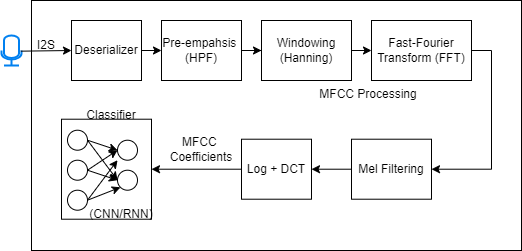
\includegraphics[width=0.45\textwidth]{figs/KWS-architecture.png}
    \caption{Keyword Spotter (KWS) architecture.}
    \label{fig:KWS_Arch}
\end{figure}

In this Section, we describe a case study of the application of our proposed design framework to the design of a digital keyword spotter system. 

Acoustic audio analysis is widely applied in critical areas such as heart monitoring, keyword spotting (KWS), and the preventive maintenance of heavy machinery \cite{chong20220}. Among these applications, KWS is essential for voice-activated assistants like Google Assistant and Amazon Alexa.

Figure~\ref{fig:KWS_Arch} depicts a widely recognized digital KWS architecture \cite{chong20220}. In this design, Mel frequency cepstral coefficients (MFCC) are used to extract spectral features from the input audio signal. 

A digital microphone captures live audio data via an I²S serial interface, which is then converted into parallel bytes. A pre-emphasis filter (high-pass filter or HPF) removes the low-frequency components of the signal. The pre-emphasis filter is typically expressed by the difference equation:
\begin{equation}
    y[n] = x[n] - \alpha~x[n-1] \label{eq:hpf}
\end{equation}
where $\alpha$ typically ranges from 0.9 to 1 \cite{han2006efficient}.

Next, a window function (e.g., Hamming or Hanning) is applied to the data to minimize spectral leakage during the FFT process. The fast Fourier transform (FFT) is then used to extract the signal’s frequency components. However, since the linear frequency scale provided by FFT does not correspond to how humans perceive sound, the linear spectrum is transformed into a Mel scale using the following equation \cite{han2006efficient}:
\begin{equation}
    Mel(f) = 2595\cdot \log_{10}\left({1 + \frac{f}{700}}\right) \label{eq:mel-log}
\end{equation}

After applying the Mel-scale transformation, the logarithm of the Mel frequency power is computed. A discrete cosine transform (DCT) is subsequently used to generate MFCC coefficients. These coefficients are then fed into a classifier, such as a convolutional neural network (CNN), recurrent neural network (RNN), or long short-term memory (LSTM) network, to recognize the keyword \cite{mahmood2021speech}. Since the classifier is hardware-intensive and computationally demanding, it is most efficiently executed on the host processor.